% Idee ja teostus: Targo Tennisberg

\documentclass[a4paper,11pt]{article}
\usepackage[et]{../../eio}
\usepackage{tikz}

\begin{document}
\begin{ol}{\eio}{\ev 8.12.2024}{\yle}{}
\begin{yl}{3}{Paberi voltimine}{volt}{1 sekund}{30 punkti}

Et kingipaberit mitte ilmaaegu kulutada, tuleb seda voltida väga täpselt. Jõuluvana abiline, noor päkapikk Krõll harjutab praegu täpset ja efektiivset voltimist, kasutades lihtsustava abivahendina ruudulist paberit ja jälgides voltimisel saadud kujundi pindala.
Täpsemalt on Krõllil $M \times N$ ruudust koosnev paberist ristkülik, mille ta kas täpselt ruudustiku joont mööda või täpselt ruutude diagonaale mööda ühe korra kokku murrab.

Lugedes koordinaatide alguspunktiks paberi vasaku alumise nurga, on murdmisjoone ja paberi servade lõikepunktide koordinaadid $(X_1, Y_1)$ ja $(X_2, Y_2)$. On teada, et kujundi pindala väheneb alati võrreldes esialgsega: murdejoon ei lange kokku paberi servaga ega puutu paberit ainult ühes punktis.

Aita Krõllil leida murdmisega saadud kujundi pindala.
  
\sis Sisendi ainsal real on kuus tühikutega eraldatud täisarvu: $M$, $N$, $X_1$, $Y_1$, $X_2$ ja $Y_2$ ($1 \le M, N \le 500$, $0 \le X_1, X_2 \le M$, $0 \le Y_1, Y_2 \le N$).

On teada, et punktid $(X_1, Y_1)$ ja $(X_2, Y_2)$ asuvad paberi servadel ja neid ühendav joon on paberi servaga kas 90- või 45-kraadise nurga all.

\val Väljundisse kirjutada pärast paberi kokkumurdmist saadud kujundi pindala.

\nde[0]{3cm}{3cm}

\begin{center}
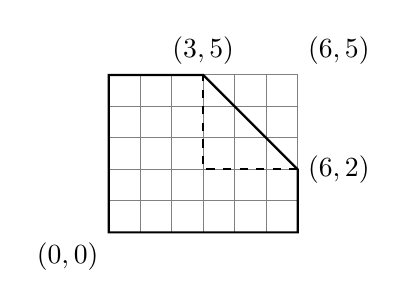
\begin{tikzpicture}[scale=0.4]
	\draw[gray] (0, 0) grid (6, 5);
	\draw[thick] (0, 0) node[below left] {$(0, 0)$};
	\draw[thick] (6, 5) node[above right] {$(6, 5)$};
	\draw[thick] (0, 0) -- (6, 0) -- (6, 2) node[right] {$(6, 2)$} -- (3, 5) node[above] {$(3, 5)$} -- (0, 5) -- cycle;
	\draw[thick, dashed] (6, 2) -- (3, 2) -- (3, 5);
\end{tikzpicture}
\end{center}

\nde[1]{3cm}{3cm}

\begin{center}
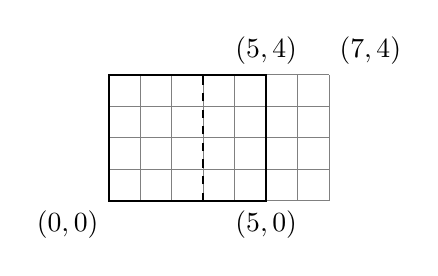
\begin{tikzpicture}[scale=0.4]
	\draw[gray] (0, 0) grid (7, 4);
	\draw[thick] (0, 0) node[below left] {$(0, 0)$};
	\draw[thick] (7, 4) node[above right] {$(7, 4)$};
	\draw[thick] (0, 0) -- (5, 0) node[below] {$(5, 0)$} -- (5, 4) node[above] {$(5, 4)$} -- (0, 4) -- cycle;
	\draw[thick, dashed] (3, 0) -- (3, 4);
\end{tikzpicture}
\end{center}

\hnd Selles ülesandes antakse punkte iga testi eest eraldi. Testid on jagatud gruppidesse, milles kehtivad järgmised lisatingimused:
\begin{xenum}
	\item (0 punkti) Ülesande tekstis olevad näited.
	\item (10 punkti) Voltimised on ainult horisontaalsed või vertikaalsed.
	\item (10 punkti) Voltimise tagajärjel tekib alati kumer hulknurk.
	\item (10 punkti) Lisapiirangud puuduvad.
\end{xenum}

\end{yl}
\end{ol}
\end{document}
